% !TEX root = saveliev_physics_general_course_2.tex
%!TEX TS-program = pdflatex
%!TEX encoding = UTF-8 Unicode


\chapter[ENERGY OF AN ELECTRIC FIELD]{ENERGY OF \\AN ELECTRIC FIELD}\label{chap:4}
\chaptermark{ENERGY OF AN ELECTRIC FIELD}


\section{Energy of a Charged Conductor}\label{sec:4_1}

The charge $q$ on a conductor can be considered as a system of point charges $\Delta{q}$. In \sect{1_7}, we obtained the following expression for the energy of interaction of a system of charges [see \eqn{1_39}]:
\begin{equation}\label{eq:4_1}
	\ab{W}{p} = \frac{1}{2} \sum_i q_i \varphi_i.
\end{equation}

\noindent
Here, $\varphi_i$ is the potential set up by all the charges except $q_i$ at the point where the charge $q_i$ is.

The surface of a conductor is equipotential. Therefore, the potentials of the points where the point charges $\Delta{q}$ are located are identical and equal the potential $\varphi$ of the conductor. Using \eqn{4_1}, we get the following expression for the energy of a charged conductor
\begin{equation}\label{eq:4_2}
	\ab{W}{p} = \frac{1}{2} \sum \varphi \Delta{q} = \frac{1}{2} \varphi \sum \Delta{q} = \frac{1}{2} \varphi q.
\end{equation}

\noindent
Taking into account \eqn{3_5}, we can write that
\begin{equation}\label{eq:4_3}
	\ab{W}{p} = \frac{\varphi q}{2} = \frac{q^2}{2 C} = \frac{C \varphi^2}{2}.
\end{equation}

\noindent
Any of these expressions gives the energy of a charged conductor.

\section{Energy of a Charged Capacitor}\label{sec:4_2}

Assume that the potential of a capacitor plate carrying the charge $+q$ is $\varphi_1$ and that of a plate carrying the charge $-q$ is $\varphi_2$. Consequently, each of the elementary charges $\Delta{q}$ into which the charge $+q$ can be divided is at a point with the potential $\varphi_1$, and each of the charges into which the charge $-q$ can be divided is at a point with the potential $\varphi_2$. By \eqn{4_1}, the energy of such a system of charges is
\begin{equation}\label{eq:4_4}
	\ab{W}{p} = \frac{1}{2} \bracket{ (+q) \varphi_1 + (-q) \varphi_2} = \frac{1}{2} q \parenthesis{\varphi_1 - \varphi_2} = \frac{1}{2} q U.
\end{equation}

\noindent
Using \eqn{3_11}, we can write three expressions for the energy of a charged capacitor:
\vspace{-12pt}
\begin{equation}\label{eq:4_5}
	\ab{W}{p} = \frac{q U}{2} = \frac{q^2}{2 C} = \frac{C U^2}{2}.
\end{equation}

\noindent
Equation \eqref{eq:4_5} differs from \eqref{eq:4_3} only in containing $U$ instead of $\varphi$.

\begin{figure}[t]
	\begin{center}
		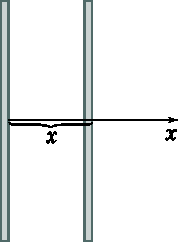
\includegraphics[scale=1]{figures/ch_04/fig_4_1.pdf}
		\caption[]{}
		\label{fig:4_1}
	\end{center}
	\vspace{-0.8cm}
\end{figure}

The expression for the potential energy permits us to find the force with which the plates of a parallel-plate capacitor attract each other. Let us assume that the separation distance of the plates can be changed. We shall associate the origin of the $x$-axis with the left-hand plate (\fig{4_1}). The coordinate $x$ of the second plate will, therefore, determine the separation distanced of the plates. According to \eqns{3_12}{4_5}, we have
\begin{equation*}
	\ab{W}{p} = \frac{q^2}{2 C} = \frac{q^2}{2 \varepsilon_0 \varepsilon S} x.
\end{equation*}

\noindent
Let us differentiate this expression with respect to $x$, assuming that the charge on the plates is constant (the capacitor is disconnected from a voltage source). As a result, we obtain the projection of the force exerted on the right-hand plate onto the $x$-axis:
\begin{equation*}
	F_x = - \diffpartial{\ab{W}{p}}{x} = - \frac{q^2}{2 \varepsilon_0 \varepsilon S}.
\end{equation*}

\noindent
The magnitude of this expression gives the force with which the plates attract each other:
\begin{equation}\label{eq:4_6}
	F = \frac{q^2}{2 \varepsilon_0 \varepsilon S}.
\end{equation}

Now, let us try to calculate the force of attraction between the plates of a parallel-plate capacitor as the product of the strength of the field produced by one of the plates and the charge concentrated on the other one. By \eqn{1_120}, the strength of the field set up by one plate is
\begin{equation}\label{eq:4_7}
	E = \frac{\sigma}{2 \varepsilon_0} = \frac{q}{2 \varepsilon_0 S}.
\end{equation}

\noindent
A dielectric weakens the field in the space between the plates $e$ times, but this occurs only inside the dielectric [see \eqn{2_33} and the related text]. The charges on the plates are outside the dielectric and are, therefore, acted upon by the field strength given by \eqn{4_7}. Multiplying the charge of a plate $q$ by this strength, we get the following expression for the force:
\begin{equation}\label{eq:4_8}
	F' = \frac{q^2}{2 \varepsilon_0 S}.
\end{equation}

Equations \eqref{eq:4_6} and \eqref{eq:4_8} do not coincide. The value of the force given by \eqn{4_6} obtained from the expression for the energy agrees with experimental data. The explanation is that apart from the ``electric'' force given by \eqn{4_8}, the plates experience mechanical forces from the side of the dielectric that tend to spread them apart (see \sect{2_8}; we must note that we have in mind a fluid dielectric). There is a dispersed field at the edges of the plates whose magnitude diminishes with an increasing distance from the edges (\fig{4_2}). The molecules of the dielectric have a dipole moment and experience the action of a force pulling them into the region with the stronger field [see \eqn{1_62}]. The result is an increase in the pressure between the plates and the appearance of a force that weakens the force given by \eqn{4_8} $e$ times.

\begin{figure}[t]
	\begin{minipage}[t]{0.48\linewidth}
		\begin{center}
			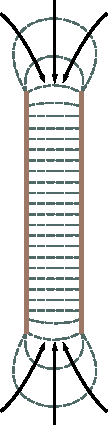
\includegraphics[scale=1]{figures/ch_04/fig_4_2.pdf}
			\caption[]{}
			\label{fig:4_2}
		\end{center}
	\end{minipage}
	\hfill{ }%space{-0.05cm}
	\begin{minipage}[t]{0.48\linewidth}
		\begin{center}
			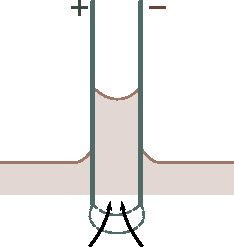
\includegraphics[scale=1]{figures/ch_04/fig_4_3.pdf}
			\caption[]{}
			\label{fig:4_3}
		\end{center}
	\end{minipage}
\vspace{-0.4cm}
\end{figure}

If a charged capacitor with an air gap is partially immersed in a liquid dielectric, the latter will be drawn into the space between the plates (\fig{4_3}). This phenomenon is explained as follows. The permittivity of air virtually equals unity. Consequently, before the plates are immersed in the dielectric, we can consider that the capacitance of the capacitor is $C_0=\varepsilon_0S/d$, and its energy is $W_0=q^2/2C_0$. When the space between the plates is partially filled with the dielectric, the capacitor can be considered as two capacitors connected in parallel, one of which has a plate area of $xS$ ($x$ is the relative part of the space filled with the liquid) and is filled with a dielectric for which $\varepsilon>1$, and the other has a plate area equal to $(1-x)S$. In the parallel connection of capacitors, their capacitances are summated:
\begin{equation*}
	C = C_1 + C_2 = \frac{\varepsilon_0 S (1-x)}{d} + \frac{\varepsilon_0 \varepsilon S x}{d} = C_0 + \frac{\varepsilon_0 (\varepsilon - 1) S}{d} x > C_0.
\end{equation*}

\noindent
Since $C>C_0$, the energy $W=q^2/2C$ will be smaller than $W_0$ (the charge $q$ is assumed to be constant---the capacitor was disconnected from the voltage source before being immersed in the liquid). Hence, the filling of the space between the plates with the dielectric is profitable from the energy viewpoint. This is why the dielectric is drawn into the capacitor and its level in the space separating the plates rises. This, in turn, results in an increase in the potential energy of gravity. In the long run, the level of the dielectric in the space will establish itself at a certain height corresponding to the minimum total energy (electrical and gravitational). The above phenomenon is similar to the capillary rise of a liquid in the narrow space between plates (see Sec. 14.5 of Vol. I).

The drawing of the dielectric into the space between plates can also be explained from the microscopic viewpoint. There is a nonuniform field at the edges of the capacitor plates. The molecules of the dielectric have an intrinsic dipole moment or acquire it under the action of the field; therefore, they experience forces that tend to transfer them to the region of the strong field, \ie, into the capacitor. These forces cause the liquid to be drawn into the space between the plates until the electric forces exerted on the liquid at the plate edges will be balanced by the weight of the liquid column.

\section{Energy of an Electric Field}\label{sec:4_3}

The energy of a charged capacitor can be expressed through quantities characterizing the electric field in the space between the plates. Let us do this for a parallel-plate capacitor. Introducing expression \eqref{eq:3_12} for the capacitance into the equation $\ab{W}{p}=CU^2/2$ [see \eqn{4_5}], we get
\begin{equation*}
	\ab{W}{p} = \frac{C U^2}{2} = \frac{\varepsilon_0 \varepsilon S U^2}{2 d} = \frac{\varepsilon_0 \varepsilon}{2} \parenthesis{\frac{U}{d}}^2 S d.
\end{equation*}

\noindent
The ratio $U/d$ equals the strength of the field between the plates; the product $Sd$ is the volume occupied by the field. Hence,
\begin{equation}\label{eq:4_9}
	\ab{W}{p} = \frac{\varepsilon_0 \varepsilon E^2}{2} V.
\end{equation}

The equation $\ab{W}{p}=q^2/(2C)$ relates the energy of a capacitor to the charge on its plates, while \eqn{4_9} relates this energy to the field strength. It is logical to ask the question: where, after all, is the energy localized (\ie, concentrated), what is the carrier of the energy---charges or a field? This question cannot be answered within the scope of electrostatics, which studies the fields of fixed charges that are constant in time. Constant fields and the charges producing them cannot exist separately from each other. Fields varying in time, however, can exist independently of the charges producing them and propagate in space in the form of electromagnetic waves. Experiments show that electromagnetic waves transfer energy. In particular, the energy due to which life exists on the Earth is supplied from the Sun by electromagnetic waves; the energy that causes a radio receiver to sound is carried from the transmitting station by electromagnetic waves, etc. These facts make us acknowledge the circumstance that the carrier of energy is a field.

If a field is homogeneous (which is the case in a parallel-plate capacitor), the energy confined in it is distributed in space with a constant density $w$ equal to the energy of the field divided by the volume it occupies. Inspection of \eqn{4_9} shows that the density of the energy of a field of strength $E$ set up in a medium with the permittivity $\varepsilon$ is
\begin{equation}\label{eq:4_10}
	w = \frac{\varepsilon_0 \varepsilon E^2}{2}.
\end{equation}

\noindent
With account taken of \eqn{2_21}, we can write \eqn{4_10} as follows:
\begin{equation}\label{eq:4_11}
	w = \frac{\varepsilon_0 \varepsilon E^2}{2} = \frac{E D}{2} = \frac{D^2}{2 \varepsilon_0 \varepsilon}.
\end{equation}

In an isotropic dielectric, the directions of the vectors $\vec{E}$ and $\vec{D}$ coincide. We can, therefore, write the equation for the energy density in the form
\begin{equation*}
	w = \frac{\vecdot{E}{D}}{2}.
\end{equation*}

\noindent
Substituting for $\vec{D}$ in this equation its value from \eqn{2_18}, we get the following expression for $w$:
\begin{equation}\label{eq:4_12}
	w = \frac{\vec{E} (\varepsilon_0 \vec{E} + \vec{P})}{2} = \frac{\varepsilon_0 \vec{E}^2}{2} + \frac{\vecdot{E}{P}}{2}.
\end{equation}

\noindent
The first addend in this expression coincides with the energy density of the field $\vec{E}$ in a vacuum. The second addend, as we shall proceed to prove, is the energy spent for polarization of the dielectric.

The polarization of a dielectric consists in that the charges contained in the molecules are displaced from their positions under the action of the electric field $\vec{E}$. The work done to displace the charges $q$, over the distance $\deriv{\vec{r}_i}$ per unit volume of the dielectric is
\begin{equation*}
	\deriv{A} = \sum_{V=i} q_i \vec{E}\, \deriv{\vec{r}_i} = \vec{E}\, \deriv\parenthesis{\sum_{V=i} q_i \vec{r}_i}
\end{equation*}

\noindent
(we consider for simplicity's sake that the field is homogeneous). According to \eqn{2_1}, $\sum_{V=i}q_i\vec{r}_i$ equals the dipole moment of a unit volume, \ie, the polarization of the dielectric $\vec{P}$. Hence,
\begin{equation}\label{eq:4_13}
	\deriv{A} = \vec{E}\, \deriv{\vec{P}}.
\end{equation}

\noindent
The vector $\vec{P}$ is related to the vector $\vec{E}$ by the expression $\vec{P}=\chi \varepsilon_0\vec{E}$ [see \eqn{2_5}]. Hence, $\deriv{\vec{P}}=\chi\varepsilon_0\, \deriv{\vec{E}}$. Using this value of $\deriv{\vec{P}}$ in \eqn{4_13}, we get the expression
\begin{equation*}
	\deriv{A} = \chi \varepsilon_0 \vec{E}\, \deriv{\vec{E}} = \deriv{\parenthesis{\frac{\chi \varepsilon_0 \vec{E}^2}{2}}} = \deriv{\parenthesis{\frac{\vecdot{E}{P}}{2}}}.
\end{equation*}

\noindent
Finally, integration gives us the following expression for the work done to polarize a unit volume of the dielectric:
\begin{equation}\label{eq:4_14}
	A = \frac{\vecdot{E}{P}}{2},
\end{equation}

\noindent
which coincides with the second addend in \eqn{4_12}. Thus, expressions \eqref{eq:4_11}, apart from the intrinsic energy of a field $\varepsilon_0 E^2/2$, include the energy $(\vecdot{E}{P})/2$ spent for the polarization of the dielectric when the field is set up.

Knowing the density of the field energy at every point, we can find the energy of the field confined in any volume $V$. For this purpose, we must calculate the integral
\begin{equation}\label{eq:4_15}
	W = \int_V w\, \deriv{V} = \int_V \frac{\varepsilon_0 \varepsilon E^2}{2}\ \deriv{V}.
\end{equation}

\noindent
Let us calculate, as an example, the energy of the field of a charged conducting sphere of radius $R$ placed in a homogeneous infinite dielectric. The field strength here is a function only of $r$:
\begin{equation*}
	E = \frac{1}{4\pi\varepsilon_0} \frac{q}{\varepsilon r^2}.
\end{equation*}

\noindent
Let us divide the space surrounding our sphere into concentric spherical layers of thickness $\deriv{r}$. The volume of a layer is $\deriv{V}=4\pi r^2\,\deriv{r}$. It contains the energy
\begin{equation*}
	\deriv{W} = w\, \deriv{V} = \frac{\varepsilon_0 \varepsilon}{2} \parenthesis{\frac{1}{4\pi\varepsilon_0} \frac{q}{\varepsilon r^2}} 4\pi r^2\,\deriv{r} = \frac{1}{2} \frac{q^2}{4\pi \varepsilon_0 \varepsilon}\, \frac{\deriv{r}}{r^2}.
\end{equation*}

\noindent
The energy of the field is
\begin{equation*}
	W =  \int \deriv{W} = \frac{1}{2} \frac{q^2}{4\pi \varepsilon_0 \varepsilon}\, \int_R^{\infty} \frac{\deriv{r}}{r^2} = \frac{1}{2} \frac{q^2}{4\pi \varepsilon_0 \varepsilon R} = \frac{q^2}{2 C}
\end{equation*}

\noindent
[according to \eqn{3_7}, $4\pi\varepsilon_0 \varepsilon R$ is the capacitance of a sphere].

The expression we have obtained coincides with that for the energy of a conductor having the capacitance $C$ and carrying the charge $q$ [see \eqn{4_3}].
